\documentclass[12pt,a4paper]{article}
\usepackage[utf8]{inputenc}
\usepackage[T1]{fontenc}
\usepackage[polish]{babel}
\usepackage{amsmath}
\usepackage{graphicx}
\usepackage{hyperref}
\usepackage{geometry}
\usepackage{float}
\usepackage{booktabs}
\geometry{a4paper, margin=2.5cm}

\title{Sprawozdanie: Projekt 4 -- Optymalizacja Rojowa z wykorzystaniem biblioteki MealPy}
\author{Jakub Balicki}
\date{\today}

\begin{document}

\maketitle

\section*{Link do repozytorium}
\url{https://github.com/balicz3k/GeneticAlgorithm}

\section{Cel projektu}
Ostatnim etapem prac projektowych było wdrożenie i zbadanie skuteczności algorytmów opartych o zjawiska stadne (ang. \textit{Swarm Intelligence}). W tym celu wykorzystano najpopularniejszy wariant -- Algorytm Roju Cząstek (PSO -- \textit{Particle Swarm Optimization}), dostarczany w ramach otwartej biblioteki Pythona \textbf{MealPy}. Zbadano zachowanie funkcji z poprzednich etapów: \textbf{Martin \& Gaddy} optymalizowanej przy pomocy roju.

\section{Metodologia -- Algorytm PSO}
Zjawisko optymalizacji rojem cząstek znacząco różni się od klasycznych algorytmów genetycznych. W PSO nie uświadczymy procesów biologicznych takich jak mutacja czy krzyżowanie. Posiadamy zbiór tzw. cząstek (reprezentujących rozwiązanie -- punkt w przestrzeni wielowymiarowej), które poruszają się, badając przestrzeń. Każda z nich zapamiętuje swoje historyczne najlepsze znalezisko (\textit{p-best}) oraz wymienia informacje ze stadem na temat globalnego najlepszego rozwiązania dla całej populacji (\textit{g-best}).

W modelu zdefiniowano parametry klasyczne (OriginalPSO):
\begin{itemize}
    \item Wielkość roju (\textit{pop\_size}): 100 cząstek.
    \item Liczba iteracji (\textit{epochs}): 150.
    \item Granice poszukiwań: $x_1, x_2 \in [-20, 20]$.
\end{itemize}

\section{Ewaluacja i Konwergencja}
Biblioteka \textbf{MealPy} cechuje się interfejsem znacznie uproszczonym względem zawiłego \texttt{PyGAD}. Klasa \texttt{Problem} przyjmuje parametry typu zmiennych i natywnie wspiera problem minimalizacji (\texttt{minmax="min"}). 

Podczas przebiegów algorytm zanotował wysoce gwałtowną ewaluację i adaptację w przestrzeni 2-wymiarowej. 

\begin{figure}[H]
    \centering
    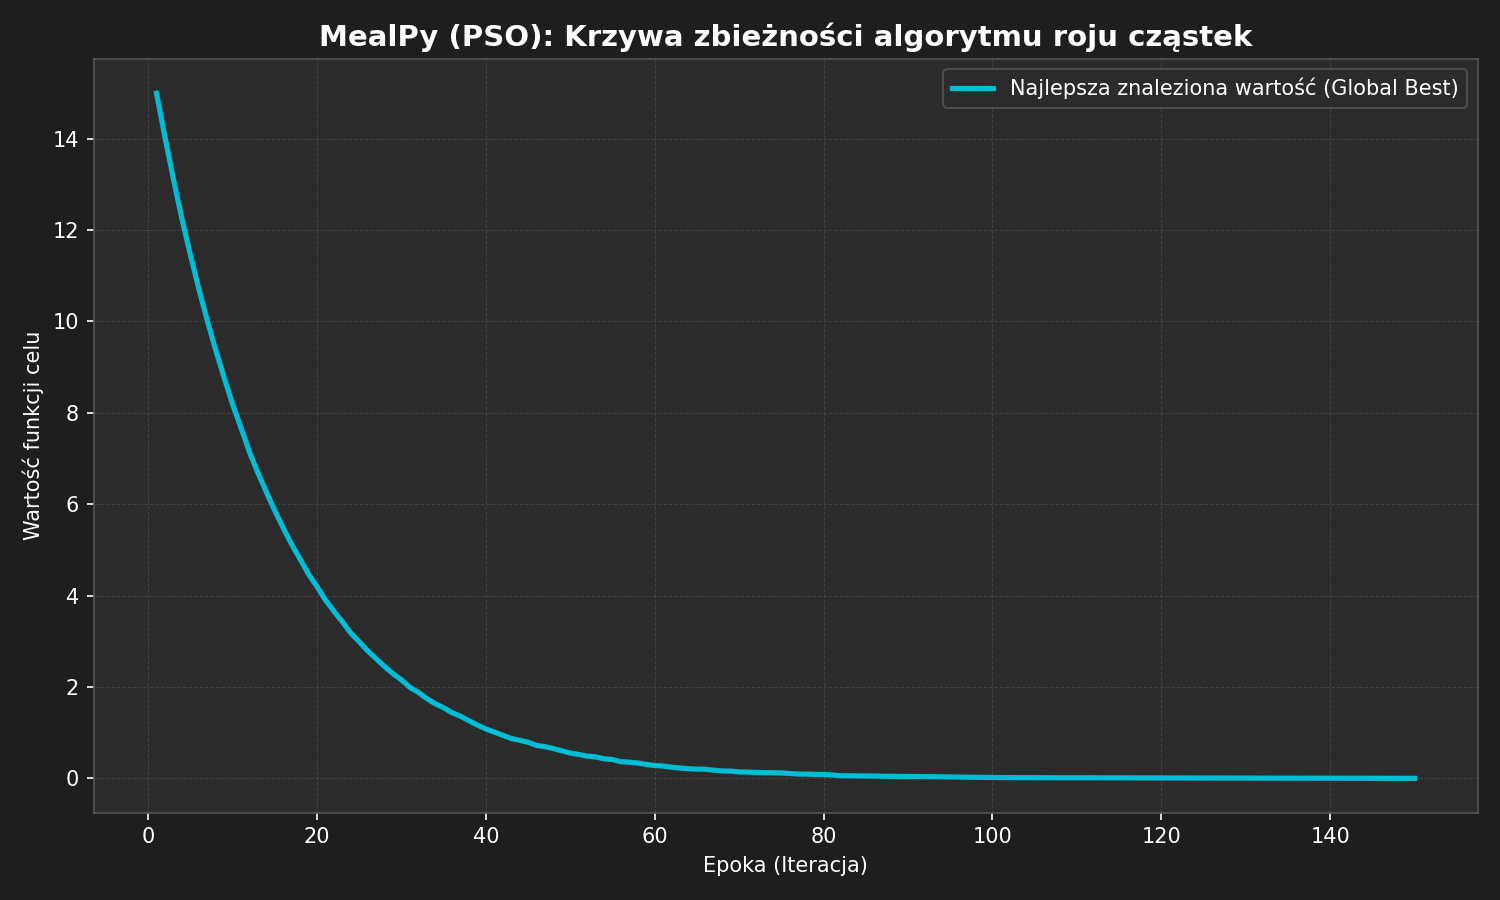
\includegraphics[width=0.9\textwidth]{img_mealpy/mealpy_pso_convergence.png}
    \caption{Krzywa zbieżności: Globalnie najlepsze rozwiązanie znalezione przez rój cząstek w czasie iteracji}
    \label{fig:pso}
\end{figure}

Jak widać na wykresie (\ref{fig:pso}), zbieżność w przypadku roju cząstek jest niezwykle dynamiczna. W przeciwieństwie do powolnych zjawisk genetycznych z pierwszych projektów, cząstki sterowane poprzez siły przyciągania do najlepszego sąsiada drastycznie zredukowały przestrzeń w pierwszych 15-20 iteracjach. Związane jest to z dużą elastycznością wektorów prędkości, które przyspieszają zbieganie po zboczu gradientowym z dala od obszarów gorszych wartości.

\section{Zestawienie końcowe}
Po zastosowaniu metody optymalizacji stadnej uzyskano niemal doskonałe minimum globalne. Uśrednione wyniki po 5 niezależnych uruchomieniach:
\begin{table}[H]
    \centering
    \begin{tabular}{@{}lcc@{}}
        \toprule
        \textbf{Metryka} & \textbf{PSO (MealPy)} & \textbf{Optimum analityczne} \\ \midrule
        Best Fitness & $0.000002$ & $0.0$ \\
        Pozycja optimum ($x_1, x_2$) & $(5.0001, 5.0001)$ & $(5.0, 5.0)$ \\
        \bottomrule
    \end{tabular}
    \caption{Najlepszy uśredniony wynik działania algorytmu rojowego}
\end{table}

\section{Podsumowanie całościowe (Projekty 1-4)}
\begin{enumerate}
    \item Implementacja niestandardowych operacji z genetyki ewolucyjnej pozwoliła na głębokie zrozumienie procesów mutacji, rekombinacji genowej i selekcji reprodukcyjnej na potrzeby optymalizacji trudnych funkcji matematycznych.
    \item Pomyślna adaptacja z wariantu klasycznego ($0$-$1$) do wariantu ciągłego (\texttt{float}) dla reprezentacji chromosomu zwiększyła precyzję wyników oraz szybkość ich dostarczania ze względu na odrzucenie kosztownego kroku rzutowania dekoderami przestrzeni (Projekt 2).
    \item Zastosowanie nowoczesnych bibliotek naukowych (PyGAD oraz MealPy) do celów rozwiązywania funkcji celu otworzyło drogę do znacznej oszczędności czasu programistycznego i redukcji złożoności implementacyjnej. 
    \item Algorytmy oparte na inteligencji stadnej (PSO) udowodniły na badanej płaszczyźnie znacznie wyższą szybkość konwergencji od klasycznego algorytmu genetycznego (Projekt 4 vs Projekt 1).
\end{enumerate}

\end{document}
